\documentclass{article}
\usepackage[utf8]{inputenc}
\usepackage[margin=0.75in]{geometry}

\title{Week 4 Class Notes}
\author{Group2: Yaxin Li, Blake Hillier, Joe Puhalla}
\date{January 2020}

\usepackage{amsmath, amssymb, amsthm}
\usepackage{graphicx}
\usepackage{wrapfig}

\begin{document}

\maketitle

\section{Support Vector Machine (SVM)}
\begin{minipage}[]{0.5\textwidth}
    Suppose we want to classify objects that are not easily separable. We could add dimensions to separate them, and then create a hyper plane between them maximizing the distance between the closest objects. In other words we want to find a point B on a hyperplane $\pi$ s.t. it is written involving $\gamma_{i}$, the maximum distance between B and the closest object from each class. 
\end{minipage}
\begin{minipage}[]{0.5\textwidth}
    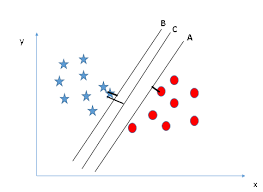
\includegraphics{Notes/svm.png}
\end{minipage}
Recall: \\
If $\vec{w}$ is a normal vector of plane $\vec{Px}$, then \begin{align*}
    \vec{Px}\perp\vec{w}=\langle\vec{Px},\vec{w}\rangle=0 \\
    \implies(x-p)\cdot=0 \\
    \implies x\vec{w}-P\vec{w}=0 \\
    \implies{w}x+b=0 \\
\end{align*}
Let's define $\gamma_{i}=y_{i}(w^{T}x+b)$. If $y_{i}=1, \ \gamma_{i}$ is large and positive, but if $y_{i}=-1, \ \gamma_{i}$ is large and negative. Now, we want $y_{i}(w^{T}x+b)\geq\gamma_{i}$ where $\|w\|=1$, which makes this optimization problem difficult. To solve this, we adjust the equation as follows: \begin{align*}
    y_{i}(\frac{\|w\|w^{T}x}{\|w\|}+b)\geq&\hat{\gamma}_{i} \\
    y_{i}(\frac{w^{T}x}{\|w\|}+\frac{b}{\|w\|})\geq&\frac{\hat{\gamma}_{i}}{w} \\
    \implies y_{i}(\hat{w}^{T}x+\hat{b})\geq&\hat{\gamma}_{i} \\
    \implies \max&\hat{\gamma}_{i} \\
\end{align*}
where $\hat{w}=\frac{w}{\|w\|}, \ \hat{b}=\frac{b}{\|w\|}$ and $\hat{\gamma}_{i}=\frac{\gamma_{i}}{\|w\|}$. Now without loss of generality, $\gamma=1$ since $\gamma=\min_{i}\{\gamma_{i}\}$. This means \begin{equation*}
    \max\hat{\sigma}\implies\max\frac{1}{\|w\|}\implies\min\|w\|\implies\min\frac{\|w\|^{2}}{2}
\end{equation*}
\end{document}
